\chapter{Conception du système}
\markboth{CHAPITRE 3. CONCEPTION DU SYSTÈME}{CHAPITRE 3. CONCEPTION DU SYSTÈME}

\section{Introduction}

La phase de conception constitue la réponse technique et architecturale aux exigences formalisées dans le chapitre précédent. Elle traduit les spécifications fonctionnelles et de cybersécurité en modèles logiciels pérennes, modulaires et directement implémentables. 

Dans ce chapitre, nous développons la modélisation dynamique de notre application logicielle (\textbf{Secure Requirements Studio -- SRS}) dédiée à l'ingénierie des exigences et à la formalisation du Cahier des Charges, à travers des diagrammes de séquences en boîte blanche, de collaboration, d'états-transitions et d'activités. Nous présentons ensuite la modélisation statique comprenant le diagramme de classes du domaine, le modèle relationnel, le dictionnaire de données exhaustif du schéma, ainsi que les architectures logicielle (diagramme de composants) et matérielle (diagramme de déploiement).

\section{Modélisation dynamique}

La modélisation dynamique décrit le comportement temporel du système, l'orchestration des flux de messages entre composants et l'évolution des états des entités au fil des interactions.

\subsection{Diagrammes de séquences}

Conformément aux préconisations d'ingénierie logicielle et aux standards EMSI, nous privilégions une représentation en \textbf{boîte blanche}, illustrant les flux internes entre le client frontend Next.js, les routeurs FastAPI, les services métier, les moteurs d'inférence et la couche de persistance.

\subsubsection{Déroulement d'un tour d'interview et dérivation d'exigences}
La figure \ref{fig:seq_interview} modélise l'enchaînement complet des traitements lors de la soumission d'une réponse par l'analyste.

\begin{figure}[H]
\centering
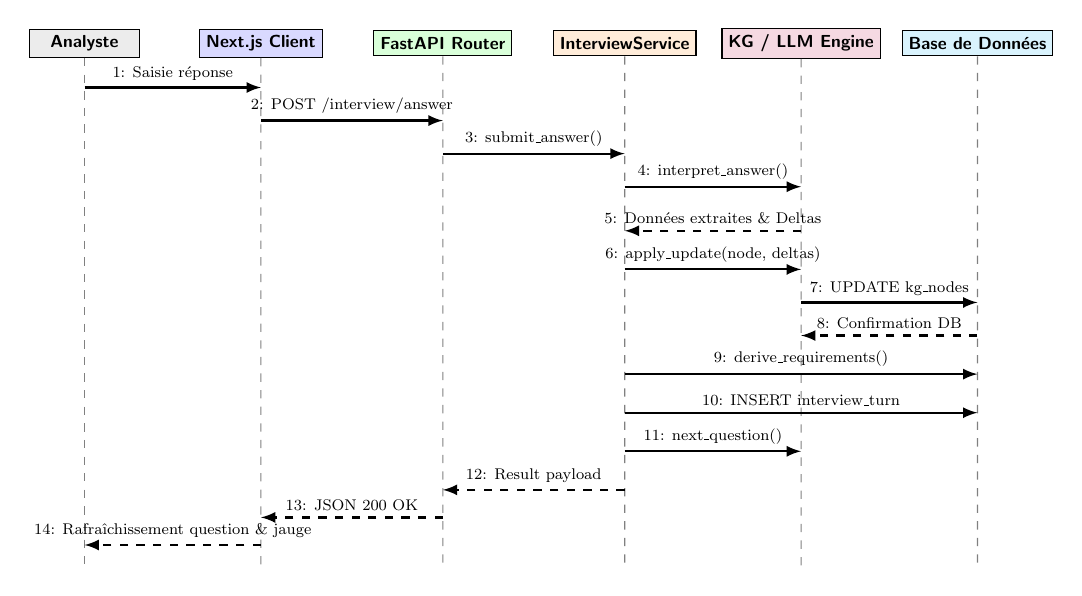
\begin{tikzpicture}[scale=0.70, every node/.style={transform shape}]
    % Lifelines headers
    \node[draw, rectangle, fill=gray!15, minimum width=2cm, font=\small\bfseries\sffamily] (user) at (0,0) {Analyste};
    \node[draw, rectangle, fill=blue!15, minimum width=2.2cm, font=\small\bfseries\sffamily] (front) at (3.2,0) {Next.js Client};
    \node[draw, rectangle, fill=green!15, minimum width=2.2cm, font=\small\bfseries\sffamily] (api) at (6.5,0) {FastAPI Router};
    \node[draw, rectangle, fill=orange!15, minimum width=2.2cm, font=\small\bfseries\sffamily] (srv) at (9.8,0) {InterviewService};
    \node[draw, rectangle, fill=purple!15, minimum width=2.2cm, font=\small\bfseries\sffamily] (kg) at (13.0,0) {KG / LLM Engine};
    \node[draw, rectangle, fill=cyan!15, minimum width=2.2cm, font=\small\bfseries\sffamily] (db) at (16.2,0) {Base de Données};

    % Lifeline dashed lines
    \draw[dashed, gray] (user) -- (0,-9.5);
    \draw[dashed, gray] (front) -- (3.2,-9.5);
    \draw[dashed, gray] (api) -- (6.5,-9.5);
    \draw[dashed, gray] (srv) -- (9.8,-9.5);
    \draw[dashed, gray] (kg) -- (13.0,-9.5);
    \draw[dashed, gray] (db) -- (16.2,-9.5);

    % Messages
    \draw[-latex, thick] (0,-0.8) -- node[above, font=\footnotesize] {1: Saisie réponse} (3.2,-0.8);
    \draw[-latex, thick] (3.2,-1.4) -- node[above, font=\footnotesize] {2: POST /interview/answer} (6.5,-1.4);
    \draw[-latex, thick] (6.5,-2.0) -- node[above, font=\footnotesize] {3: submit\_answer()} (9.8,-2.0);
    
    \draw[-latex, thick] (9.8,-2.6) -- node[above, font=\footnotesize] {4: interpret\_answer()} (13.0,-2.6);
    \draw[dashed, -latex, thick] (13.0,-3.4) -- node[above, font=\footnotesize] {5: Données extraites \& Deltas} (9.8,-3.4);

    \draw[-latex, thick] (9.8,-4.1) -- node[above, font=\footnotesize] {6: apply\_update(node, deltas)} (13.0,-4.1);
    \draw[-latex, thick] (13.0,-4.7) -- node[above, font=\footnotesize] {7: UPDATE kg\_nodes} (16.2,-4.7);
    \draw[dashed, -latex, thick] (16.2,-5.3) -- node[above, font=\footnotesize] {8: Confirmation DB} (13.0,-5.3);

    \draw[-latex, thick] (9.8,-6.0) -- node[above, font=\footnotesize] {9: derive\_requirements()} (16.2,-6.0);
    \draw[-latex, thick] (9.8,-6.7) -- node[above, font=\footnotesize] {10: INSERT interview\_turn} (16.2,-6.7);
    \draw[-latex, thick] (9.8,-7.4) -- node[above, font=\footnotesize] {11: next\_question()} (13.0,-7.4);

    \draw[dashed, -latex, thick] (9.8,-8.1) -- node[above, font=\footnotesize] {12: Result payload} (6.5,-8.1);
    \draw[dashed, -latex, thick] (6.5,-8.6) -- node[above, font=\footnotesize] {13: JSON 200 OK} (3.2,-8.6);
    \draw[dashed, -latex, thick] (3.2,-9.1) -- node[above, font=\footnotesize] {14: Rafraîchissement question \& jauge} (0,-9.1);
\end{tikzpicture}
\caption{Diagramme de séquence en boîte blanche : Traitement d'un tour d'interview}
\label{fig:seq_interview}
\end{figure}

\subsubsection{Génération et assemblage du document de spécification}
La figure \ref{fig:seq_docgen} illustre la séquence d'assemblage multi-sources menée par le service de génération documentaire pour produire le cahier des charges officiel.

\begin{figure}[H]
\centering
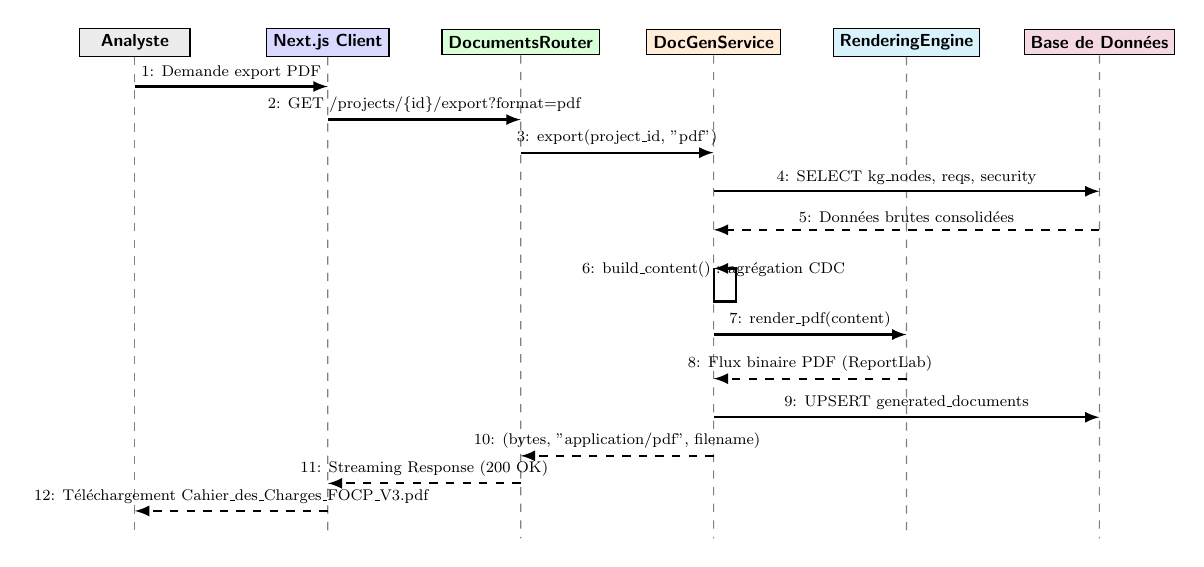
\begin{tikzpicture}[scale=0.70, every node/.style={transform shape}]
    % Lifelines
    \node[draw, rectangle, fill=gray!15, minimum width=2cm, font=\small\bfseries\sffamily] (user) at (0,0) {Analyste};
    \node[draw, rectangle, fill=blue!15, minimum width=2.2cm, font=\small\bfseries\sffamily] (front) at (3.5,0) {Next.js Client};
    \node[draw, rectangle, fill=green!15, minimum width=2.2cm, font=\small\bfseries\sffamily] (api) at (7.0,0) {DocumentsRouter};
    \node[draw, rectangle, fill=orange!15, minimum width=2.2cm, font=\small\bfseries\sffamily] (docgen) at (10.5,0) {DocGenService};
    \node[draw, rectangle, fill=cyan!15, minimum width=2.2cm, font=\small\bfseries\sffamily] (render) at (14.0,0) {RenderingEngine};
    \node[draw, rectangle, fill=purple!15, minimum width=2.2cm, font=\small\bfseries\sffamily] (db) at (17.5,0) {Base de Données};

    % Dashed lines
    \draw[dashed, gray] (user) -- (0,-9.0);
    \draw[dashed, gray] (front) -- (3.5,-9.0);
    \draw[dashed, gray] (api) -- (7.0,-9.0);
    \draw[dashed, gray] (docgen) -- (10.5,-9.0);
    \draw[dashed, gray] (render) -- (14.0,-9.0);
    \draw[dashed, gray] (db) -- (17.5,-9.0);

    % Sequence
    \draw[-latex, thick] (0,-0.8) -- node[above, font=\footnotesize] {1: Demande export PDF} (3.5,-0.8);
    \draw[-latex, thick] (3.5,-1.4) -- node[above, font=\footnotesize] {2: GET /projects/\{id\}/export?format=pdf} (7.0,-1.4);
    \draw[-latex, thick] (7.0,-2.0) -- node[above, font=\footnotesize] {3: export(project\_id, "pdf")} (10.5,-2.0);

    \draw[-latex, thick] (10.5,-2.7) -- node[above, font=\footnotesize] {4: SELECT kg\_nodes, reqs, security} (17.5,-2.7);
    \draw[dashed, -latex, thick] (17.5,-3.4) -- node[above, font=\footnotesize] {5: Données brutes consolidées} (10.5,-3.4);

    \draw[-latex, thick] (10.5,-4.1) -- node[above, font=\footnotesize] {6: build\_content() : agrégation CDC} (10.5,-4.7) -- (10.9,-4.7) -- (10.9,-4.1) -- (10.5,-4.1);

    \draw[-latex, thick] (10.5,-5.3) -- node[above, font=\footnotesize] {7: render\_pdf(content)} (14.0,-5.3);
    \draw[dashed, -latex, thick] (14.0,-6.1) -- node[above, font=\footnotesize] {8: Flux binaire PDF (ReportLab)} (10.5,-6.1);

    \draw[-latex, thick] (10.5,-6.8) -- node[above, font=\footnotesize] {9: UPSERT generated\_documents} (17.5,-6.8);

    \draw[dashed, -latex, thick] (10.5,-7.5) -- node[above, font=\footnotesize] {10: (bytes, "application/pdf", filename)} (7.0,-7.5);
    \draw[dashed, -latex, thick] (7.0,-8.0) -- node[above, font=\footnotesize] {11: Streaming Response (200 OK)} (3.5,-8.0);
    \draw[dashed, -latex, thick] (3.5,-8.5) -- node[above, font=\footnotesize] {12: Téléchargement Cahier\_des\_Charges\_FOCP\_V3.pdf} (0,-8.5);
\end{tikzpicture}
\caption{Diagramme de séquence : Génération et exportation du Cahier des Charges}
\label{fig:seq_docgen}
\end{figure}

\subsection{Diagrammes de collaboration}

Le diagramme de collaboration met l'accent sur l'organisation structurelle des objets échangeant des messages lors de l'exécution d'un audit qualité par le moteur de revue. La figure \ref{fig:collab_review} illustre cette orchestration.

\begin{figure}[H]
\centering
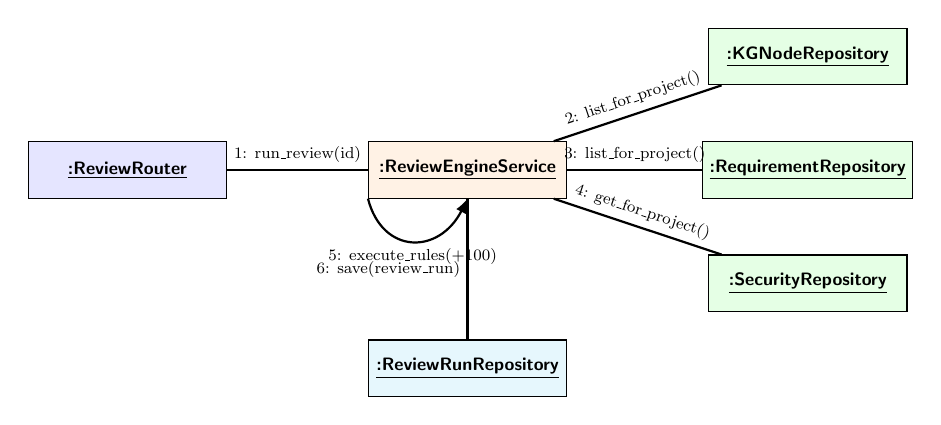
\begin{tikzpicture}[scale=0.72, every node/.style={transform shape}]
    % Objects
    \node[draw, rectangle, fill=blue!10, minimum width=3.5cm, minimum height=1cm, align=center, font=\small\sffamily] (router) at (0,4) {\textbf{\underline{:ReviewRouter}}};
    \node[draw, rectangle, fill=orange!10, minimum width=3.5cm, minimum height=1cm, align=center, font=\small\sffamily] (service) at (6,4) {\textbf{\underline{:ReviewEngineService}}};
    \node[draw, rectangle, fill=green!10, minimum width=3.5cm, minimum height=1cm, align=center, font=\small\sffamily] (repo_kg) at (12,6) {\textbf{\underline{:KGNodeRepository}}};
    \node[draw, rectangle, fill=green!10, minimum width=3.5cm, minimum height=1cm, align=center, font=\small\sffamily] (repo_req) at (12,4) {\textbf{\underline{:RequirementRepository}}};
    \node[draw, rectangle, fill=green!10, minimum width=3.5cm, minimum height=1cm, align=center, font=\small\sffamily] (repo_sec) at (12,2) {\textbf{\underline{:SecurityRepository}}};
    \node[draw, rectangle, fill=cyan!10, minimum width=3.5cm, minimum height=1cm, align=center, font=\small\sffamily] (run_repo) at (6,0.5) {\textbf{\underline{:ReviewRunRepository}}};

    % Links
    \draw[thick] (router) -- node[above, font=\footnotesize] {1: run\_review(id)} (service);
    \draw[thick] (service) -- node[above, sloped, font=\footnotesize] {2: list\_for\_project()} (repo_kg);
    \draw[thick] (service) -- node[above, font=\footnotesize] {3: list\_for\_project()} (repo_req);
    \draw[thick] (service) -- node[above, sloped, font=\footnotesize] {4: get\_for\_project()} (repo_sec);
    \draw[thick] (service) -- node[left, font=\footnotesize] {6: save(review\_run)} (run_repo);

    % Self loop for rule execution
    \draw[thick, -latex] (service.south west) .. controls (4.5,2.5) and (5.5,2.5) .. node[below, font=\footnotesize] {5: execute\_rules(+100)} (service.south);
\end{tikzpicture}
\caption{Diagramme de collaboration : Exécution de l'audit qualité et cybersécurité}
\label{fig:collab_review}
\end{figure}

\needspace{14\baselineskip}
\subsection{Diagrammes d'états et d'état-transition}

Le cycle de vie d'un projet de spécification est gouverné par un automate fini garantissant que les étapes d'élicitation, de revue et de validation sont franchies avec rigueur. La figure \ref{fig:state_project} présente le diagramme d'état-transition d'un projet.

\begin{figure}[H]
\centering
\begin{tikzpicture}[scale=0.84, transform shape,
    state_box/.style={draw=emsiblue, fill=white, rounded corners=8pt, line width=1.1pt, minimum width=3.4cm, minimum height=1.3cm, align=center, font=\small\sffamily},
    trans/.style={-latex, thick, draw=emsiblue, line width=1pt, font=\scriptsize\sffamily},
    cond/.style={font=\tiny\bfseries\itshape\color{focpgreendark}},
    err_trans/.style={-latex, thick, dashed, draw=red!70!black, line width=1pt, font=\scriptsize\sffamily}
]
    % Nodes
    \node[draw=focpgreendark, circle, fill=focpgreendark, minimum size=0.5cm] (init) at (0,0) {};
    
    \node[state_box, fill=blue!3] (brouillon) at (3.6,0) {
        \textbf{\color{emsiblue}Brouillon}\\[2pt]
        \footnotesize 0\% complétude\\
        \tiny Métadonnées \& ontologie 39
    };
    
    \node[state_box, fill=orange!5] (en_cours) at (9.2,0) {
        \textbf{\color{orange!80!black}En cours}\\[2pt]
        \footnotesize Interview active\\
        \tiny Enrichissement dynamique du KG
    };
    
    \node[state_box, fill=purple!5] (en_revue) at (9.2,-3.6) {
        \textbf{\color{purple!80!black}En revue}\\[2pt]
        \footnotesize Audit qualité\\
        \tiny Évaluation des +100 règles
    };
    
    \node[state_box, fill=focpgreenlight] (valide) at (3.6,-3.6) {
        \textbf{\color{focpgreendark}Validé}\\[2pt]
        \footnotesize Score global $\ge 95\%$\\
        \tiny Homologation formelle
    };
    
    \node[draw=focpgreendark, double, circle, fill=focpgreendark, minimum size=0.5cm] (final) at (0,-3.6) {};

    % Transitions
    \draw[trans] (init) -- node[above] {Création} (brouillon);
    \draw[trans] (brouillon) -- node[above] {Démarrage interview} (en_cours);
    \draw[trans] (en_cours.east) .. controls (12.2, 0.8) and (12.2, -0.8) .. node[right, align=left, font=\tiny] {Tour validé \&\\mise à jour KG} (en_cours.east);
    \draw[trans] (en_cours) -- node[right] {Interview complétée} (en_revue);
    \draw[trans] (en_revue) -- node[above] {Audit réussi} node[below, cond] {[Score $\ge 95\%$]} (valide);
    \draw[err_trans] (en_revue) -- node[above, sloped, color=red!70!black] {Lacunes / échec} node[below, sloped, font=\tiny\itshape\color{red!70!black}] {[Score $< 95\%$]} (en_cours);
    \draw[trans] (valide) -- node[above] {Export CDC final} (final);
\end{tikzpicture}
\caption{Diagramme d'état-transition du cycle de vie d'un projet de spécification}
\label{fig:state_project}
\end{figure}

\needspace{14\baselineskip}
\subsection{Diagrammes d'activité}

La figure \ref{fig:activity_interview} modélise l'activité globale d'administration d'une session d'interview et de propagation des connaissances capturées.

\begin{figure}[H]
\centering
\begin{tikzpicture}[scale=0.85, every node/.style={transform shape}]
    % Nodes
    \node[draw, circle, fill=black, minimum size=0.4cm] (start) at (0,0) {};
    \node[draw, rectangle, rounded corners, fill=gray!10, minimum width=4cm, font=\footnotesize\sffamily, align=center] (a1) at (0,-1.0) {Charger le graphe de connaissances};
    \node[draw, diamond, fill=yellow!15, aspect=2, font=\footnotesize\sffamily, align=center] (d1) at (0,-2.5) {Mode IA ou\\Classique ?};
    \node[draw, rectangle, rounded corners, fill=purple!10, minimum width=3.5cm, font=\footnotesize\sffamily, align=center] (a2_ai) at (-3,-3.8) {Formulation IA (Gemini)};
    \node[draw, rectangle, rounded corners, fill=blue!10, minimum width=3.5cm, font=\footnotesize\sffamily, align=center] (a2_cl) at (3,-3.8) {Banque de questions guidée};
    \node[draw, rectangle, rounded corners, fill=gray!10, minimum width=4cm, font=\footnotesize\sffamily, align=center] (a3) at (0,-5.0) {Afficher la question \& recueillir la réponse};
    \node[draw, rectangle, rounded corners, fill=gray!10, minimum width=4cm, font=\footnotesize\sffamily, align=center] (a4) at (0,-6.2) {Interpréter la réponse \& mettre à jour le noeud KG};
    \node[draw, rectangle, rounded corners, fill=gray!10, minimum width=4cm, font=\footnotesize\sffamily, align=center] (a5) at (0,-7.4) {Dériver automatiquement les exigences associées};
    \node[draw, diamond, fill=yellow!15, aspect=2, font=\footnotesize\sffamily, align=center] (d2) at (0,-8.8) {Reste-t-il des\\concepts incomplets ?};
    \node[draw, rectangle, rounded corners, fill=green!15, minimum width=4cm, font=\footnotesize\sffamily, align=center] (a6) at (0,-10.2) {Clôturer l'interview \& notifier l'analyste};
    \node[draw, double, circle, fill=black!70, minimum size=0.4cm] (end) at (0,-11.2) {};

    % Arrows
    \draw[-latex, thick] (start) -- (a1);
    \draw[-latex, thick] (a1) -- (d1);
    \draw[-latex, thick] (d1) -| node[above, font=\scriptsize] {[Mode IA]} (a2_ai);
    \draw[-latex, thick] (d1) -| node[above, font=\scriptsize] {[Mode Classique]} (a2_cl);
    \draw[-latex, thick] (a2_ai) |- (a3);
    \draw[-latex, thick] (a2_cl) |- (a3);
    \draw[-latex, thick] (a3) -- (a4);
    \draw[-latex, thick] (a4) -- (a5);
    \draw[-latex, thick] (a5) -- (d2);
    \draw[-latex, thick] (d2) -- node[right, font=\scriptsize] {[Non]} (a6);
    \draw[-latex, thick] (d2.east) -- ++(3.5,0) |- node[near start, right, font=\scriptsize] {[Oui]} (a1.east);
    \draw[-latex, thick] (a6) -- (end);
\end{tikzpicture}
\caption{Diagramme d'activité : Processus d'interview et dérivation des exigences}
\label{fig:activity_interview}
\end{figure}

\section{Modélisation statique}

La modélisation statique formalise la structure logique des données, les classes d'entités, leurs attributs, leurs méthodes et leurs relations.

\subsection{Diagramme de classes du domaine}

La figure \ref{fig:class_diagram} présente le diagramme de classes UML représentant fidèlement les modèles ORM SQLAlchemy implémentés dans le backend de notre application logicielle SRS.

\begin{figure}[H]
\centering
\begin{tikzpicture}[scale=0.75, every node/.style={transform shape}]
    % Project Class
    \node[draw, rectangle, fill=blue!10, minimum width=4.5cm, align=left, font=\scriptsize\sffamily] (project) at (0,6) {
        \textbf{\large Project}\\
        \rule{4cm}{0.4pt}\\
        + id : UUID [PK]\\
        + name : String(300)\\
        + short\_name : String(120)\\
        + department : String(200)\\
        + description : Text\\
        + status : String(30)\\
        + progress : Integer\\
        + security\_score : Integer\\
        + organization\_id : UUID [FK]\\
        + created\_at : DateTime\\
        \rule{4cm}{0.4pt}\\
        + calculate\_progress() : int\\
        + update\_status(new\_status)
    };

    % KG Node Class
    \node[draw, rectangle, fill=orange!10, minimum width=4.5cm, align=left, font=\scriptsize\sffamily] (kg_node) at (7,8.5) {
        \textbf{\large KnowledgeGraphNode}\\
        \rule{4cm}{0.4pt}\\
        + id : UUID [PK]\\
        + project\_id : UUID [FK]\\
        + concept\_key : String(150)\\
        + domain : String(30)\\
        + label : String(300)\\
        + completion : Integer\\
        + confidence : Integer\\
        + importance : String(20)\\
        + captured\_data : JSON\\
        + missing\_information : JSON\\
        \rule{4cm}{0.4pt}\\
        + apply\_delta(comp, conf)\\
        + is\_sufficient() : bool
    };

    % Requirement Class
    \node[draw, rectangle, fill=green!10, minimum width=4.5cm, align=left, font=\scriptsize\sffamily] (req) at (7,3.5) {
        \textbf{\large Requirement}\\
        \rule{4cm}{0.4pt}\\
        + id : UUID [PK]\\
        + project\_id : UUID [FK]\\
        + requirement\_key : String(20)\\
        + requirement\_type : String(30)\\
        + title : String(300)\\
        + priority : String(20)\\
        + actors : JSON\\
        + acceptance\_criteria : JSON\\
        + security\_controls : JSON\\
        + source\_concept\_key : String(150)\\
        \rule{4cm}{0.4pt}\\
        + validate\_traceability() : bool
    };

    % Interview Session Class
    \node[draw, rectangle, fill=purple!10, minimum width=4.2cm, align=left, font=\scriptsize\sffamily] (session) at (-6,8.5) {
        \textbf{\large InterviewSession}\\
        \rule{4cm}{0.4pt}\\
        + id : UUID [PK]\\
        + project\_id : UUID [FK]\\
        + status : String(20)\\
        + pending\_concept\_key : String(150)\\
        + pending\_question : Text\\
        \rule{4cm}{0.4pt}\\
        + next\_turn()\\
        + close\_session()
    };

    % Interview Turn Class
    \node[draw, rectangle, fill=purple!5, minimum width=4.2cm, align=left, font=\scriptsize\sffamily] (turn) at (-6,3.5) {
        \textbf{\large InterviewTurn}\\
        \rule{4cm}{0.4pt}\\
        + id : UUID [PK]\\
        + session\_id : UUID [FK]\\
        + sequence : Integer\\
        + question : Text\\
        + answer : Text\\
        + completion\_delta : Integer\\
        + consultant\_note : Text\\
        + extracted\_data : JSON\\
        \rule{4cm}{0.4pt}
    };

    % Security Analysis Class
    \node[draw, rectangle, fill=red!10, minimum width=4.5cm, align=left, font=\scriptsize\sffamily] (sec) at (-3,-1) {
        \textbf{\large SecurityAnalysis}\\
        \rule{4cm}{0.4pt}\\
        + id : UUID [PK]\\
        + project\_id : UUID [FK, Unique]\\
        + threat\_model : JSON\\
        + rbac\_matrix : JSON\\
        + risk\_register : JSON\\
        + privacy\_impact\_assessment : JSON\\
        + security\_score : Integer\\
        \rule{4cm}{0.4pt}\\
        + evaluate\_stride()\\
        + calculate\_score() : int
    };

    % Review Run Class
    \node[draw, rectangle, fill=yellow!15, minimum width=4.5cm, align=left, font=\scriptsize\sffamily] (review) at (3.5,-1) {
        \textbf{\large ReviewRun}\\
        \rule{4cm}{0.4pt}\\
        + id : UUID [PK]\\
        + project\_id : UUID [FK, Unique]\\
        + findings : JSON\\
        + rule\_count : Integer\\
        + failed\_count : Integer\\
        + overall\_score : Integer\\
        + approved\_for\_export : Boolean\\
        \rule{4cm}{0.4pt}\\
        + execute\_rules()\\
        + check\_approval() : bool
    };

    % Generated Document Class
    \node[draw, rectangle, fill=cyan!10, minimum width=4.5cm, align=left, font=\scriptsize\sffamily] (doc) at (10,-1) {
        \textbf{\large GeneratedDocument}\\
        \rule{4cm}{0.4pt}\\
        + id : UUID [PK]\\
        + project\_id : UUID [FK, Unique]\\
        + content : JSON\\
        + created\_at : DateTime\\
        \rule{4cm}{0.4pt}\\
        + render\_pdf() : bytes\\
        + render\_docx() : bytes
    };

    % Relationships
    \draw[thick, -diamond] (project) -- node[above, font=\scriptsize] {1\quad\quad\quad 0..*} (kg_node);
    \draw[thick, -diamond] (project) -- node[above, font=\scriptsize] {1\quad\quad\quad 0..*} (req);
    \draw[thick, -diamond] (project) -- node[above, font=\scriptsize] {1\quad\quad\quad 0..1} (session);
    \draw[thick, -diamond] (session) -- node[right, font=\scriptsize] {1\quad 0..*} (turn);
    \draw[thick, -diamond] (project) -- node[left, font=\scriptsize] {1\quad 0..1} (sec);
    \draw[thick, -diamond] (project) -- node[right, font=\scriptsize] {1\quad 0..1} (review);
    \draw[thick, -diamond] (project) -- node[right, font=\scriptsize] {1\quad 0..1} (doc);
    \draw[thick, dashed, -latex] (kg_node) -- node[right, font=\scriptsize] {$\ll$traces\_to$\gg$} (req);
\end{tikzpicture}
\caption{Diagramme de classes du domaine de l'application de formalisation des exigences}
\label{fig:class_diagram}
\end{figure}

\subsection{Modèle relationnel}

Le passage du modèle conceptuel au modèle relationnel s'appuie sur les règles canoniques de dérivation de l'ingénierie des bases de données :
\begin{enumerate}
    \item Chaque entité devient une table relationnelle dotée d'une clé primaire UUID non prédictible.
    \item Les relations de composition $1 \rightarrow N$ (ex. : \texttt{Project} $\rightarrow$ \texttt{Requirements}) se traduisent par une clé étrangère (\texttt{project\_id}) dans la table fille avec suppression en cascade (\texttt{ON DELETE CASCADE}).
    \item Les relations $1 \rightarrow 1$ (ex. : \texttt{Project} $\rightarrow$ \texttt{SecurityAnalysis}, \texttt{GeneratedDocument}) sont modélisées par une clé étrangère assortie d'une contrainte d'unicité (\texttt{UNIQUE}).
    \item Les structures semi-dynamiques (matrices RBAC, règles de validation) sont encapsulées dans des colonnes natives \texttt{JSON}.
\end{enumerate}

Le schéma relationnel textuel s'exprime comme suit :
\begin{flushleft}
\small
\begin{itemize}
    \item \textbf{organizations} (\underline{id}, name, slug, created\_at, updated\_at)
    \item \textbf{users} (\underline{id}, email, hashed\_password, full\_name, is\_active, is\_superuser, created\_at, updated\_at)
    \item \textbf{projects} (\underline{id}, name, short\_name, department, description, status, progress, security\_score, \textit{organization\_id}, \textit{owner\_id}, created\_at, updated\_at)
    \item \textbf{knowledge\_graph\_nodes} (\underline{id}, \textit{project\_id}, concept\_key, domain, label, description, completion, confidence, importance, business\_value, risk, status, validation\_rules, missing\_information, captured\_data, generated\_questions, created\_at, updated\_at)
    \item \textbf{knowledge\_graph\_edges} (\underline{id}, \textit{node\_id}, \textit{dependency\_node\_id}, created\_at, updated\_at)
    \item \textbf{interview\_sessions} (\underline{id}, \textit{project\_id}, status, pending\_concept\_key, pending\_question, created\_at, updated\_at)
    \item \textbf{interview\_turns} (\underline{id}, \textit{session\_id}, sequence, concept\_key, question, answer, completion\_delta, confidence\_delta, consultant\_note, extracted\_data, created\_at, updated\_at)
    \item \textbf{requirements} (\underline{id}, \textit{project\_id}, requirement\_key, requirement\_type, title, description, priority, business\_goal, risk, status, owner, actors, acceptance\_criteria, dependencies, security\_controls, database\_tables, api\_endpoints, ui\_screens, test\_cases, source\_concept\_key, created\_at, updated\_at)
    \item \textbf{security\_analyses} (\underline{id}, \textit{project\_id}, threat\_model, rbac\_matrix, risk\_register, security\_checklist, privacy\_impact\_assessment, data\_classification, security\_score, created\_at, updated\_at)
    \item \textbf{review\_runs} (\underline{id}, \textit{project\_id}, findings, rule\_count, failed\_count, completeness\_score, confidence\_score, security\_score, architecture\_score, business\_score, testing\_score, overall\_score, approved\_for\_export, created\_at, updated\_at)
    \item \textbf{generated\_documents} (\underline{id}, \textit{project\_id}, content, created\_at, updated\_at)
\end{itemize}
\end{flushleft}

\subsection{Dictionnaire de données}

Le tableau \ref{tab:data_dict} synthétise le dictionnaire de données exhaustif extrait du schéma physique effectif de notre base de données.

\begin{table}[H]
\centering
\caption{Dictionnaire de données du schéma de la base de données}
\label{tab:data_dict}
\resizebox{\textwidth}{!}{%
\begin{tabular}{|l|l|l|c|l|l|c|c|l|}
\hline
\rowcolor{focpgreen!18}
\textbf{Nom colonne} & \textbf{Type} & \textbf{Taille} & \textbf{Oblig.} & \textbf{Défaut} & \textbf{Valeurs autorisées} & \textbf{PK} & \textbf{FK} & \textbf{Nom table} \\
\hline
id & UUID & 36 car. & Oui & uuid4() & Chaîne UUID v4 & Oui & Non & projects \\
name & String & 300 car. & Oui & Aucun & Texte & Non & Non & projects \\
short\_name & String & 120 car. & Oui & Aucun & Texte & Non & Non & projects \\
department & String & 200 car. & Oui & "" & Texte & Non & Non & projects \\
status & String & 30 car. & Oui & "brouillon" & brouillon, en\_cours, en\_revue, valide & Non & Non & projects \\
progress & Integer & 4 octets & Oui & 0 & 0 à 100 & Non & Non & projects \\
security\_score & Integer & 4 octets & Oui & 0 & 0 à 100 & Non & Non & projects \\
organization\_id & UUID & 36 car. & Oui & Aucun & Référence organizations.id & Non & Oui & projects \\
owner\_id & UUID & 36 car. & Oui & Aucun & Référence users.id & Non & Oui & projects \\
\hline
id & UUID & 36 car. & Oui & uuid4() & Chaîne UUID v4 & Oui & Non & knowledge\_graph\_nodes \\
project\_id & UUID & 36 car. & Oui & Aucun & Référence projects.id & Non & Oui & knowledge\_graph\_nodes \\
concept\_key & String & 150 car. & Oui & Aucun & Clé ontologique (ex. business.objective) & Non & Non & knowledge\_graph\_nodes \\
domain & String & 30 car. & Oui & Aucun & business, users, security, deployment, etc. & Non & Non & knowledge\_graph\_nodes \\
completion & Integer & 4 octets & Oui & 0 & 0 à 100 & Non & Non & knowledge\_graph\_nodes \\
confidence & Integer & 4 octets & Oui & 0 & 0 à 100 & Non & Non & knowledge\_graph\_nodes \\
captured\_data & JSON & Variable & Oui & \{\} & Objet JSON structuré & Non & Non & knowledge\_graph\_nodes \\
\hline
id & UUID & 36 car. & Oui & uuid4() & Chaîne UUID v4 & Oui & Non & requirements \\
project\_id & UUID & 36 car. & Oui & Aucun & Référence projects.id & Non & Oui & requirements \\
requirement\_key & String & 20 car. & Oui & Aucun & Ex. BR-001, FR-002, SEC-003 & Non & Non & requirements \\
requirement\_type & String & 30 car. & Oui & Aucun & business, functional, security, technical & Non & Non & requirements \\
priority & String & 20 car. & Oui & "medium" & low, medium, high, critical & Non & Non & requirements \\
source\_concept\_key & String & 150 car. & Oui & Aucun & Référence concept\_key & Non & Non & requirements \\
\hline
id & UUID & 36 car. & Oui & uuid4() & Chaîne UUID v4 & Oui & Non & security\_analyses \\
project\_id & UUID & 36 car. & Oui & Aucun & Référence projects.id (Unique) & Non & Oui & security\_analyses \\
threat\_model & JSON & Variable & Oui & [] & Liste des menaces STRIDE & Non & Non & security\_analyses \\
rbac\_matrix & JSON & Variable & Oui & \{\} & Matrice rôles/ressources & Non & Non & security\_analyses \\
security\_score & Integer & 4 octets & Oui & 0 & 0 à 100 & Non & Non & security\_analyses \\
\hline
id & UUID & 36 car. & Oui & uuid4() & Chaîne UUID v4 & Oui & Non & review\_runs \\
project\_id & UUID & 36 car. & Oui & Aucun & Référence projects.id (Unique) & Non & Oui & review\_runs \\
overall\_score & Integer & 4 octets & Oui & 0 & 0 à 100 & Non & Non & review\_runs \\
approved\_for\_export & Boolean & 1 octet & Oui & False & True / False & Non & Non & review\_runs \\
\hline
id & UUID & 36 car. & Oui & uuid4() & Chaîne UUID v4 & Oui & Non & generated\_documents \\
project\_id & UUID & 36 car. & Oui & Aucun & Référence projects.id (Unique) & Non & Oui & generated\_documents \\
content & JSON & Variable & Oui & \{\} & Arborescence documentaire complète & Non & Non & generated\_documents \\
\hline
\end{tabular}%
}
\end{table}

\subsection{Architecture de l'application}

\subsubsection{Architecture logicielle (Diagramme de composants)}
L'architecture logicielle globale de l'application développée est structurée selon le paradigme multicouche découplé et asynchrone, représenté à la figure \ref{fig:component_diag}.

\begin{figure}[H]
\centering
\begin{tikzpicture}[scale=0.76, transform shape,
    layer_pkg/.style={draw=emsiblue, fill=blue!2, rounded corners=6pt, line width=1pt, inner sep=8pt},
    comp/.style={draw=emsiblue, fill=white, rounded corners=4pt, line width=0.8pt, font=\scriptsize\sffamily, align=center, minimum height=0.9cm, text width=2.5cm},
    data_comp/.style={draw=focpgreendark, fill=focpgreenlight, rounded corners=4pt, line width=0.8pt, font=\scriptsize\sffamily, align=center, minimum height=0.9cm, text width=2.6cm},
    ext_comp/.style={draw=purple!80, fill=purple!5, rounded corners=4pt, line width=0.9pt, font=\scriptsize\bfseries\sffamily, align=center, minimum height=0.9cm, text width=2.6cm},
    conn/.style={-latex, thick, draw=emsiblue, line width=0.9pt},
    data_conn/.style={-latex, thick, draw=focpgreendark, line width=0.9pt},
    ext_conn/.style={-latex, dashed, thick, draw=purple!80, line width=0.9pt}
]
    % Layer 1: Frontend
    \draw[layer_pkg] (-0.2, 7.2) rectangle (15.2, 9.6);
    \node[anchor=north west, font=\footnotesize\bfseries\sffamily\color{emsiblue}] at (0.0, 9.4) {1. Couche Présentation (Next.js 15 App Router / React 19 / Tailwind v4)};
    \node[comp] (f_ui) at (1.6, 8.2) {UI Design System\\(Composants \& Thèmes)};
    \node[comp] (f_wiz) at (5.3, 8.2) {Interview Stepper\\(Wizard interactif)};
    \node[comp] (f_dash) at (9.0, 8.2) {Dashboard \&\\Visualisation KG};
    \node[comp] (f_api) at (13.0, 8.2) {API Client Typed\\(Fetch / REST)};

    % Layer 2: API Gateway / Routing
    \draw[layer_pkg] (-0.2, 4.4) rectangle (15.2, 6.4);
    \node[anchor=north west, font=\footnotesize\bfseries\sffamily\color{emsiblue}] at (0.0, 6.2) {2. Couche Exposition API \& Validation (FastAPI / Pydantic v2)};
    \node[comp, text width=4.0cm] (b_router) at (4.0, 5.2) {API Routers REST\\(/projects, /interview, /review)};
    \node[comp, text width=4.0cm] (b_schema) at (11.0, 5.2) {Pydantic v2 Schemas\\(Validation stricte \& Typage)};

    % Layer 3: Business Domain Engines
    \draw[layer_pkg] (-0.2, 1.4) rectangle (15.2, 3.8);
    \node[anchor=north west, font=\footnotesize\bfseries\sffamily\color{emsiblue}] at (0.0, 3.6) {3. Couche Métier \& Moteurs Spécialisés (Python 3.12)};
    \node[comp, text width=2.4cm] (b_int) at (1.5, 2.4) {Interview Engine\\(Dual-Mode)};
    \node[comp, text width=2.4cm] (b_kg) at (4.5, 2.4) {Knowledge Graph\\(39 Concepts)};
    \node[comp, text width=2.4cm] (b_sec) at (7.6, 2.4) {Security Engine\\(STRIDE / RBAC)};
    \node[comp, text width=2.4cm] (b_rev) at (10.7, 2.4) {Review Engine\\(+100 Règles)};
    \node[comp, text width=2.4cm] (b_doc) at (13.7, 2.4) {Doc Generator\\(PDF / DOCX)};

    % Layer 4: Persistence
    \draw[layer_pkg, draw=focpgreen, fill=focpgreenlight!20] (-0.2, -1.6) rectangle (10.2, 0.8);
    \node[anchor=north west, font=\footnotesize\bfseries\sffamily\color{focpgreendark}] at (0.0, 0.6) {4. Couche Données \& Persistance (SQLAlchemy 2.0 Async)};
    \node[data_comp] (b_orm) at (2.2, -0.6) {Async Repositories\\(CRUD \& Queries)};
    \node[draw=focpgreendark, cylinder, shape border rotate=90, aspect=0.25, fill=white, line width=0.9pt, font=\scriptsize\bfseries\sffamily\color{focpgreendark}, align=center] (b_db) at (7.5, -0.6) {PostgreSQL 16\\/ SQLite (Local)};

    % External Service
    \draw[draw=purple!80, fill=purple!2, rounded corners=6pt, line width=1pt] (10.8, -1.6) rectangle (15.2, 0.8);
    \node[anchor=north west, font=\footnotesize\bfseries\sffamily\color{purple!80!black}] at (11.0, 0.6) {Services Cloud Externes};
    \node[ext_comp] (ext_ai) at (13.0, -0.6) {Google Gemini API\\(SDK GenAI Cloud)};

    % Intra-layer frontend
    \draw[conn] (f_wiz) -- (f_ui);
    \draw[conn] (f_wiz) -- (f_api);
    \draw[conn] (f_dash) -- (f_api);

    % Frontend -> API
    \draw[conn, line width=1.1pt] (f_api.south) -- node[right, font=\scriptsize\bfseries] {HTTPS / JSON} (b_schema.north -| f_api.south);

    % API -> Schemas
    \draw[conn] (b_router) -- (b_schema);

    % API -> Domain Engines
    \draw[conn] (b_router.south) -- (b_kg.north);
    \draw[conn] (b_router.south) -- (b_int.north);
    \draw[conn] (b_router.south) -- (b_sec.north);
    \draw[conn] (b_router.south) -- (b_rev.north);
    \draw[conn] (b_router.south) -- (b_doc.north);

    % Domain inter-engine flows
    \draw[conn] (b_int) -- (b_kg);
    \draw[conn] (b_kg) -- (b_sec);
    \draw[conn] (b_sec) -- (b_rev);
    \draw[conn] (b_rev) -- (b_doc);

    % Domain -> Data
    \draw[data_conn] (b_kg.south) -- (b_orm.north -| b_kg.south);
    \draw[data_conn] (b_orm) -- (b_db);

    % Interview -> AI
    \draw[ext_conn] (b_int.south) -- ++(0,-0.6) -| (ext_ai.north);

\end{tikzpicture}
\caption{Diagramme de composants de l'architecture logicielle (SRS)}
\label{fig:component_diag}
\end{figure}

\clearpage
\subsubsection{Architecture matérielle (Diagramme de déploiement)}

La topologie de déploiement de la solution logicielle \textbf{SRS} repose sur une architecture conteneurisée trois tiers orchestrée par \textbf{Docker Compose}, garantissant l'isolation des services, la portabilité multi-environnements et la persistance des données. 

Le diagramme de déploiement UML de la figure \ref{fig:deployment_diag} explicite les n{\oe}uds matériels (\textit{devices}), les environnements d'exécution (\textit{execution environments}), les conteneurs et les flux de communication :

\begin{itemize}[leftmargin=1.0cm, label=\textcolor{focpgreen}{$\bullet$}]
    \item \textbf{Tier Client} ($\ll$device$\gg$ Poste Client) : Navigateur web moderne exécutant l'application monopage (SPA) Next.js 15, React 19 et Tailwind CSS v4.
    \item \textbf{Tier Applicatif} ($\ll$device$\gg$ Serveur Hôte) : Écosystème Docker Compose encapsulant les conteneurs Frontend (Node.js 24), Backend (FastAPI / Python 3.12) et Base de données (PostgreSQL 16 avec volume persistant \texttt{postgres\_data}).
    \item \textbf{Tier Cloud Externe} ($\ll$cloud$\gg$ Google Cloud) : Service Google AI Studio fournissant l'accès aux modèles Gemini 1.5 via API REST sécurisée en HTTPS / TLS 1.3.
\end{itemize}

\vspace{0.2cm}

\begin{figure}[H]
\centering
\begin{tikzpicture}[scale=0.70, transform shape,
    % --- Styles des Nœuds UML ---
    device_node/.style={
        draw=emsiblue, fill=blue!3, rounded corners=8pt,
        line width=1.2pt, font=\sffamily
    },
    docker_host_node/.style={
        draw=focpgreendark, fill=focpgreenlight!12, rounded corners=8pt,
        line width=1.3pt, font=\sffamily
    },
    cloud_node/.style={
        draw=purple!85!black, fill=purple!4, rounded corners=8pt,
        line width=1.2pt, font=\sffamily, align=center
    },
    card_node/.style={
        draw=emsiblue!80, fill=white, rounded corners=5pt,
        line width=0.8pt, font=\sffamily, align=center,
        drop shadow={opacity=0.06, shadow xshift=1pt, shadow yshift=-1pt}
    },
    db_card_node/.style={
        draw=focpgreendark, fill=white, rounded corners=5pt,
        line width=0.8pt, font=\sffamily, align=center,
        drop shadow={opacity=0.06, shadow xshift=1pt, shadow yshift=-1pt}
    },
    artifact_node/.style={
        draw=gray!50, fill=gray!3, rounded corners=4pt,
        line width=0.6pt, font=\sffamily, align=center
    },
    % --- Styles des connecteurs ---
    flow_blue/.style={-latex, line width=1.0pt, draw=emsiblue},
    flow_green/.style={-latex, line width=1.0pt, draw=focpgreendark},
    flow_purple/.style={-latex, dashed, line width=1.0pt, draw=purple!85!black},
    lbl/.style={
        fill=white, inner sep=2.5pt, rounded corners=2pt,
        draw=gray!35, line width=0.4pt, font=\tiny\bfseries\sffamily
    }
]

    % =========================================================================
    % 1. POSTE CLIENT (Gauche : x de 0 à 3.6)
    % =========================================================================
    \draw[device_node] (0, -4.5) rectangle (3.6, 4.5);
    \node[anchor=north, font=\sffamily, align=center] at (1.8, 4.3) {
        {\scriptsize\color{emsiblue}$\ll$device$\gg$}\\[1pt]
        \textbf{\normalsize\color{emsiblue}Poste Client}\\[1pt]
        {\tiny\color{black!70}Navigateur Web (Chrome/Firefox)}
    };

    % Artifact SPA
    \node[artifact_node, text width=2.8cm, minimum height=5.0cm] (spa) at (1.8, -0.7) {
        \textbf{\scriptsize $\ll$artifact$\gg$}\\[2pt]
        \textbf{\normalsize SPA Frontend}\\[3pt]
        {\footnotesize Next.js 15 App Router}\\[2pt]
        {\scriptsize React 19 $\;\cdot\;$ TypeScript}\\[2pt]
        {\scriptsize Tailwind CSS v4}\\[6pt]
        \rule{2.2cm}{0.4pt}\\[4pt]
        {\tiny\color{black!70} Rendu IHM \& Wizard}\\[2pt]
        {\tiny\color{black!70} Knowledge Graph Visualizer}\\[2pt]
        {\tiny\color{black!70} Client d'API Typé (Fetch)}
    };

    % =========================================================================
    % 2. SERVEUR D'APPLICATION HÔTE (Centre : x de 5.0 à 14.6)
    % =========================================================================
    \draw[docker_host_node] (5.0, -4.5) rectangle (14.6, 4.5);
    \node[anchor=north, font=\sffamily, align=center] at (9.8, 4.3) {
        {\scriptsize\color{focpgreendark}$\ll$device / server$\gg$}\\[1pt]
        \textbf{\normalsize\color{focpgreendark}Serveur d'Application Hôte}\\[1pt]
        {\tiny\bfseries\color{focpgreendark!80}Écosystème Docker Compose (Réseau privé bridgé)}
    };

    % Conteneur 1 : Frontend
    \node[card_node, text width=7.8cm, minimum height=1.3cm] (c_front) at (10.2, 2.1) {
        \textbf{\scriptsize\color{emsiblue}$\ll$container$\gg$ frontend}\\[2pt]
        \textbf{\footnotesize Node.js 24 Alpine} $\;\cdot\;$ \texttt{Port d'écoute : 3000}\\[1pt]
        {\tiny Serveur Next.js (Rendu SSR, API Routes \& Reverse Proxy)}
    };

    % Conteneur 2 : Backend
    \node[card_node, text width=7.8cm, minimum height=1.5cm] (c_back) at (10.2, -0.3) {
        \textbf{\scriptsize\color{srsaccent}$\ll$container$\gg$ backend}\\[2pt]
        \textbf{\footnotesize Python 3.12 / FastAPI + Uvicorn} $\;\cdot\;$ \texttt{Port : 8000}\\[1pt]
        {\tiny Moteurs : Élicitation IA, Ontologie (39 concepts), STRIDE/RBAC, Audit Qualité}
    };

    % Conteneur 3 : Database
    \node[db_card_node, text width=7.8cm, minimum height=1.3cm] (c_db) at (10.2, -2.7) {
        \textbf{\scriptsize\color{focpgreendark}$\ll$container$\gg$ database}\\[2pt]
        \textbf{\footnotesize PostgreSQL 16 Alpine} $\;\cdot\;$ \texttt{Port interne : 5432}\\[1pt]
        {\tiny Volume persistant hôte : \texttt{postgres\_data} $\;\cdot\;$ Pilote \texttt{asyncpg}}
    };

    % =========================================================================
    % 3. GOOGLE CLOUD PLATFORM (Droite : x de 15.6 à 19.6)
    % =========================================================================
    \draw[cloud_node] (15.6, -1.8) rectangle (19.6, 1.2);
    \node[anchor=north, font=\sffamily, align=center] at (17.6, 1.0) {
        {\scriptsize\color{purple!80!black}$\ll$cloud service$\gg$}\\[1pt]
        \textbf{\normalsize\color{purple!80!black}Google Cloud}\\[2pt]
        {\footnotesize\bfseries\color{black!80}Google AI Studio}\\[4pt]
        {\scriptsize\bfseries API Gemini 1.5 Pro / Flash}\\[2pt]
        {\tiny\color{black!70}Inférence LLM adaptative}
    };

    % =========================================================================
    % 4. CONNECTEURS ET PROTOCOLES
    % =========================================================================
    % 4.1 Client -> Frontend (HTTP 3000)
    \draw[flow_blue] (3.6, 2.1) -- (6.3, 2.1)
        node[midway, lbl, above=1pt] {HTTP :3000};

    % 4.2 Client -> Backend (REST 8000)
    \draw[flow_blue] (3.6, -0.3) -- (6.3, -0.3)
        node[midway, lbl, above=1pt] {REST :8000};

    % 4.3 Frontend -> Backend (Proxy API interne via bus latéral gauche)
    \draw[flow_blue] (6.3, 1.5) -- ++(-0.8, 0) |- (6.3, 0.3)
        node[pos=0.25, lbl, left=1pt] {Proxy API :8000};

    % 4.4 Backend -> Database (TCP asyncpg via bus latéral gauche)
    \draw[flow_green] (6.3, -0.9) -- ++(-0.8, 0) |- (6.3, -2.1)
        node[pos=0.25, lbl, left=1pt] {TCP 5432};

    % 4.5 Backend -> Google Cloud (HTTPS TLS 1.3)
    \draw[flow_purple] (14.1, -0.3) -- (15.6, -0.3)
        node[midway, lbl, above=1pt, align=center] {HTTPS TLS 1.3\\[-1pt]\tiny(API Key)};

\end{tikzpicture}
\caption[Diagramme de déploiement de l'application SRS]{Diagramme de déploiement de l'application logicielle développée (SRS)}
\label{fig:deployment_diag}
\end{figure}

\needspace{8\baselineskip}
\section{Conclusion}

Ce chapitre a détaillé la conception architecturale, dynamique et statique de notre application logicielle SRS. La modélisation UML rigoureuse illustre l'orchestration des flux entre les moteurs d'élicitation, de cybersécurité et de génération documentaire. Le modèle relationnel et son dictionnaire de données traduisent fidèlement l'implémentation de la base de données. Le chapitre suivant présente l'environnement de développement, la réalisation des interfaces graphiques de SRS et l'analyse du livrable final obtenu.

\newpage
